\lecture_date{08/11/2026}
\chapter{Lecture 08}

\section{Automatic differentiation}
Lecture 07 covered numerical differentiation and complex step. We now compute derivatives directly using the chain rule, without choosing a step size.

\begin{definition}[Automatic differentiation]
Automatic differentiation (AD) evaluates derivatives of a computation by decomposing it into elementary operations with known derivative rules and systematically applying the chain rule to those operations.
\end{definition}
AD computes the gradient at a specified point from the operations defining the function. Its derivatives are exact up to machine precision: there is no finite-step approximation error, but floating-point rounding remains.

There are two main modes: \emph{forward accumulation} and \emph{reverse accumulation} (reverse-mode AD). Both use the same chain rule; their propagation directions differ. This lecture develops reverse mode. The forward-mode algorithm is left for the next lecture.

\subsection{Reverse-mode AD}
A computational graph is a directed acyclic graph. Inputs are source nodes; each later node represents an elementary operation on earlier nodes. An arrow $a\to b$ means that $b$ directly uses $a$. Forward evaluation follows the arrows in topological order, so every operand is available before it is used.

\subsubsection*{The six steps}
\begin{enumerate}
\item \textbf{Generate the computational graph.} Break the expression into elementary operations and draw their dependencies.
\item \textbf{Name the intermediate nodes.} Assign a variable to each intermediate result; reuse a node when its value is used again.
\item \textbf{Calculate intermediate node values.} Substitute the input point and evaluate forward, including the output.
\item \textbf{Write local derivatives.} For each operation, differentiate its output with respect to each immediate operand, holding its other operands fixed.
\item \textbf{Calculate derivative values.} Evaluate these local derivatives using the forward values.
\item \textbf{Reverse accumulation.} Seed the scalar output derivative with one, then propagate derivatives backward, adding contributions whenever a value is used along more than one path.
\end{enumerate}
Steps 3--5 can be combined in a forward pass. Step 6 is the reverse pass.

\subsubsection*{Local and accumulated derivatives}
For an edge $a\to b$, write $\partial b/\partial a$ for the \emph{local} derivative of that operation. Define the \emph{adjoint}
\[
 \bar a:=\frac{\partial f}{\partial a},
\]
meaning the sensitivity of the final scalar output through \emph{all} downstream uses of $a$. This distinction is crucial when the graph branches.

Initially set all adjoints to zero and set $\bar f=1$. Process operation nodes $b$ in reverse topological order. For each operand $a$ of $b$, perform
\begin{equation}
 \boxed{\bar a\mathrel{+}=\bar b\,\frac{\partial b}{\partial a}.}
 \label{eq:lec08-update}
\end{equation}
Here $+=$ means \emph{add to the existing value}. If a node has several outgoing paths, add their contributions.

Thus we multiply along a path and sum over distinct paths. Reverse topological order ensures that a node has received every downstream contribution before its adjoint is propagated farther backward. At the end, $\nabla f=(\bar x_1,\ldots,\bar x_n)^T$.

\begin{example}[A logarithm of a sum]
Find the gradient of
\[
 f(x_1,x_2,x_3)=\ln(x_1x_2+x_3^2)
 \quad\text{at }(1,1,1).
\]
\end{example}

Here $\log$ means the natural logarithm $\ln$, whose derivative is $1/v$. The input to $\ln$ must be positive.

\subsubsection*{Steps 1--3: graph and forward evaluation}
Set $u_1=x_1x_2$, $u_2=x_3^2$, $v=u_1+u_2$ and $f=\ln v$.
\begin{center}
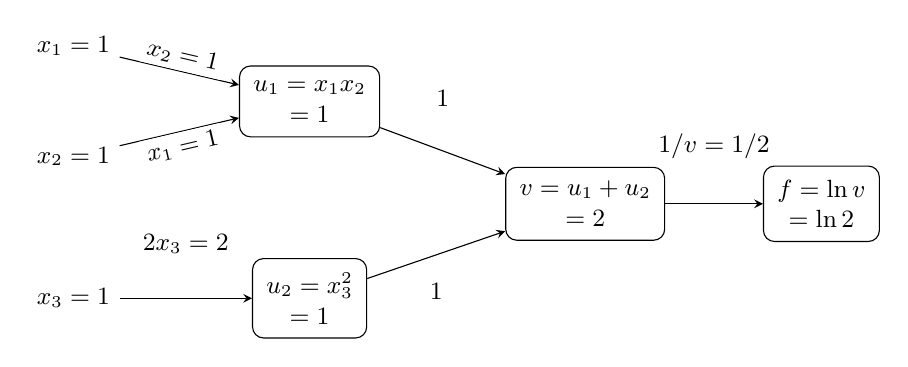
\begin{tikzpicture}[>=stealth, every node/.style={font=\small},
 op/.style={draw,rounded corners,align=center,minimum height=9mm,inner sep=5pt},
 lab/.style={fill=white,inner sep=2pt,font=\small}]
\node (x1) at (0,2) {$x_1=1$};
\node (x2) at (0,0.6) {$x_2=1$};
\node (x3) at (0,-1.2) {$x_3=1$};
\node[op] (u1) at (3,1.3) {$u_1=x_1x_2$\\$=1$};
\node[op] (u2) at (3,-1.2) {$u_2=x_3^2$\\$=1$};
\node[op] (v) at (6.5,0) {$v=u_1+u_2$\\$=2$};
\node[op] (f) at (9.5,0) {$f=\ln v$\\$=\ln2$};
\draw[->] (x1)--node[lab,above,sloped] {$x_2=1$} (u1);
\draw[->] (x2)--node[lab,below,sloped] {$x_1=1$} (u1);
\draw[->] (x3)--node[lab,above=14pt] {$2x_3=2$} (u2);
\draw[->] (u1)--node[lab,above=14pt] {$1$} (v);
\draw[->] (u2)--node[lab,below=8pt] {$1$} (v);
\draw[->] (v)--node[lab,above=14pt] {$1/v=1/2$} (f);
\end{tikzpicture}

\small Arrows show forward dependencies. Each edge label is the local derivative of its destination with respect to its source, evaluated at the given point.
\end{center}
The forward values are
\[
 (x_1,x_2,x_3)=(1,1,1),\qquad
 (u_1,u_2,v,f)=(1,1,2,\ln2).
\]

\subsubsection*{Steps 4--5: local edge derivatives}
\begin{center}
\renewcommand{\arraystretch}{1.25}
\begin{tabular}{lll}
\toprule
Edge & Local derivative & Value\\
\midrule
$x_1\to u_1$ & $\partial u_1/\partial x_1=x_2$ & $1$\\
$x_2\to u_1$ & $\partial u_1/\partial x_2=x_1$ & $1$\\
$x_3\to u_2$ & $\partial u_2/\partial x_3=2x_3$ & $2$\\
$u_1\to v$ & $\partial v/\partial u_1=1$ & $1$\\
$u_2\to v$ & $\partial v/\partial u_2=1$ & $1$\\
$v\to f$ & $\partial f/\partial v=1/v$ & $1/2$\\
\bottomrule
\end{tabular}
\end{center}
Differentiate the operation first, then substitute its operands. Replacing $u_2=x_3^2$ by the evaluated number $1$ before differentiating would lose its dependence on $x_3$.

\subsubsection*{Step 6: reverse adjoints}
Start at the output and work backward:
\begin{align*}
 \bar f&=1,\\
 \bar v&=\bar f\frac{\partial f}{\partial v}
       =1\cdot\frac12=\frac12,\\
 \bar u_1&=\bar v\frac{\partial v}{\partial u_1}
       =\frac12\cdot1=\frac12,\\
 \bar u_2&=\bar v\frac{\partial v}{\partial u_2}
       =\frac12\cdot1=\frac12,\\
 \bar x_1&=\bar u_1\frac{\partial u_1}{\partial x_1}
       =\frac12\cdot1=\frac12,\\
 \bar x_2&=\bar u_1\frac{\partial u_1}{\partial x_2}
       =\frac12\cdot1=\frac12,\\
 \bar x_3&=\bar u_2\frac{\partial u_2}{\partial x_3}
       =\frac12\cdot2=1.
\end{align*}
Therefore,
\[
 \boxed{\nabla f(1,1,1)=\begin{bmatrix}1/2\\1/2\\1\end{bmatrix}.}
\]
Each input here has only one path to the output. For example,
\[
 \frac{\partial f}{\partial x_3}
 =\frac{\partial f}{\partial v}
  \frac{\partial v}{\partial u_2}
  \frac{\partial u_2}{\partial x_3}
 =\frac12\cdot1\cdot2=1.
\]
The reverse pass reuses already accumulated quantities such as $\bar v$, rather than recomputing the entire path product for each input.

\clearpage
\begin{example}[A shared intermediate value]
Consider
\[
 f(x_1,x_2)=x_1x_2\exp\bigl(\sin(x_1x_2)\bigr)
 \quad\text{at }(1,0).
\]
\end{example}

Define $u=x_1x_2$, $v=\sin u$, $w=e^v$ and $f=uw$. The same $u$ is used both in $\sin u$ and in the final multiplication. It must have two outgoing edges.

\subsubsection*{Forward values and local derivatives}
\begin{center}
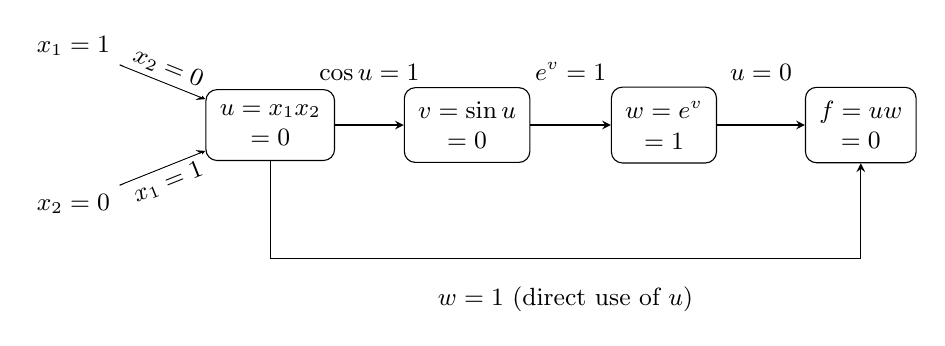
\begin{tikzpicture}[>=stealth,every node/.style={font=\small},
 op/.style={draw,rounded corners,align=center,minimum height=9mm,inner sep=5pt},
 lab/.style={fill=white,inner sep=2pt,font=\small}]
\node (x1) at (0,1) {$x_1=1$};
\node (x2) at (0,-1) {$x_2=0$};
\node[op] (u) at (2.5,0) {$u=x_1x_2$\\$=0$};
\node[op] (v) at (5,0) {$v=\sin u$\\$=0$};
\node[op] (w) at (7.5,0) {$w=e^v$\\$=1$};
\node[op] (f) at (10,0) {$f=uw$\\$=0$};
\draw[->] (x1)--node[lab,above,sloped] {$x_2=0$} (u);
\draw[->] (x2)--node[lab,below,sloped] {$x_1=1$} (u);
\draw[->] (u)--node[lab,above=14pt] {$\cos u=1$} (v);
\draw[->] (v)--node[lab,above=14pt] {$e^v=1$} (w);
\draw[->] (w)--node[lab,above=14pt] {$u=0$} (f);
\draw[->] (u.south)--(2.5,-1.7)--node[lab,below=8pt] {$w=1$ (direct use of $u$)} (10,-1.7)--(f.south);
\end{tikzpicture}

\small Forward dependencies with evaluated local derivatives on the edges.
\end{center}
The forward pass gives $(u,v,w,f)=(0,0,1,0)$. All local derivatives are listed explicitly below.
\begin{center}
\renewcommand{\arraystretch}{1.3}
\begin{tabular}{lll}
\toprule
Edge & Local derivative & Value\\
\midrule
$x_1\to u$ & $\partial u/\partial x_1=x_2$ & $0$\\
$x_2\to u$ & $\partial u/\partial x_2=x_1$ & $1$\\
$u\to v$ & $\partial v/\partial u=\cos u$ & $1$\\
$v\to w$ & $\partial w/\partial v=e^v$ & $1$\\
$w\to f$ & $\left.\partial(uw)/\partial w\right|_u=u$ & $0$\\
$u\to f$ & $\left.\partial(uw)/\partial u\right|_w=w$ & $1$\\
\bottomrule
\end{tabular}
\end{center}
The subscript on the last two derivatives identifies the operand held fixed. The direct edge derivative $\left.\partial(uw)/\partial u\right|_w=w$ is only one contribution to $\bar u$. Globally, $w=e^{\sin u}$ also depends on $u$.

\subsubsection*{Reverse accumulation: add both contributions}
Seed $\bar f=1$. A valid reverse order is $f,w,v,u,x_2,x_1$:
\begin{align*}
 \bar w&=\bar f\,u=1\cdot0=0,\\
 \bar v&=\bar w\,e^v=0\cdot1=0,\\
 \bar u&=\underbrace{\bar f\,w}_{\text{direct path }u\to f}
       +\underbrace{\bar v\,\cos u}_{\text{path }u\to v\to w\to f}
       =1\cdot1+0\cdot1=1,\\
 \bar x_1&=\bar u\,x_2=1\cdot0=0,\\
 \bar x_2&=\bar u\,x_1=1\cdot1=1.
\end{align*}
Hence
\[
 \boxed{\nabla f(1,0)=\begin{bmatrix}0\\1\end{bmatrix}.}
\]
An implementation first adds $1$ to $\bar u$ through the direct edge when processing $f$. Later, when processing $v$, it adds $0$. It must not overwrite the existing $1$ with $0$.

\subsubsection*{Why the two contributions are added}
The direct edge $u\to f$ differentiates $uw$ holding $w$ fixed, giving $w$. The other path accounts for $w=e^{\sin u}$ also changing with $u$. Together they give the product rule:
\[
 \bar u=w+u\,e^{\sin u}\cos u=1+0=1\quad\text{at }u=0.
\]
The local edge derivative and the accumulated derivative are different quantities. This distinction resolves the notation difficulty discussed in class.

\begin{example}[Two paths from the same input]
Find the gradient of
\[
 f(x_1,x_2)=x_1^2+\sin(x_1x_2),\qquad (x_1,x_2)=(1,0).
\]
\end{example}

Set $u_1=x_1^2$, $u_2=x_1x_2$, $v=\sin u_2$ and $f=u_1+v$. Now the input $x_1$ itself branches.
\begin{center}
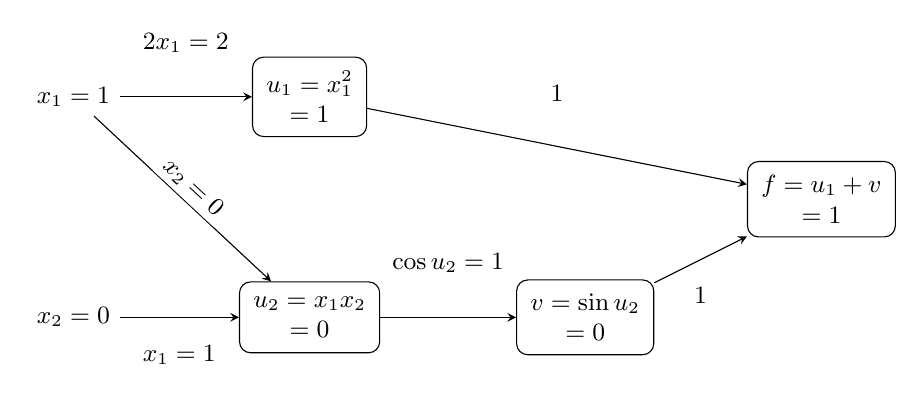
\begin{tikzpicture}[>=stealth,every node/.style={font=\small},
 op/.style={draw,rounded corners,align=center,minimum height=9mm,inner sep=5pt},
 lab/.style={fill=white,inner sep=2pt,font=\small}]
\node (x1) at (0,1.3) {$x_1=1$};
\node (x2) at (0,-1.5) {$x_2=0$};
\node[op] (u1) at (3,1.3) {$u_1=x_1^2$\\$=1$};
\node[op] (u2) at (3,-1.5) {$u_2=x_1x_2$\\$=0$};
\node[op] (v) at (6.5,-1.5) {$v=\sin u_2$\\$=0$};
\node[op] (f) at (9.5,0) {$f=u_1+v$\\$=1$};
\draw[->] (x1)--node[lab,above=14pt] {$2x_1=2$} (u1);
\draw[->] (x1)--node[lab,above,sloped] {$x_2=0$} (u2);
\draw[->] (x2)--node[lab,below=8pt] {$x_1=1$} (u2);
\draw[->] (u2)--node[lab,above=14pt] {$\cos u_2=1$} (v);
\draw[->] (u1)--node[lab,above=14pt] {$1$} (f);
\draw[->] (v)--node[lab,below=8pt] {$1$} (f);
\end{tikzpicture}

\small Node values and all six evaluated local edge derivatives.
\end{center}
The forward values are $(u_1,u_2,v,f)=(1,0,0,1)$. In reverse, seed $\bar f=1$, then obtain
\[
 \bar u_1=\bar f\cdot1=1,\qquad
 \bar v=\bar f\cdot1=1,\qquad
 \bar u_2=\bar v\cos u_2=1.
\]
Both children of $x_1$ must contribute:
\begin{align*}
 \bar x_1
 &=\bar u_1\frac{\partial u_1}{\partial x_1}
  +\bar u_2\frac{\partial u_2}{\partial x_1}
  =1\cdot2+1\cdot0=2,\\
 \bar x_2&=\bar u_2\frac{\partial u_2}{\partial x_2}=1\cdot1=1.
\end{align*}
Thus $\boxed{\nabla f(1,0)=(2,1)^T}$. Written as full path products,
\[
 \frac{\partial f}{\partial x_1}
 =\underbrace{\frac{\partial f}{\partial u_1}
   \frac{\partial u_1}{\partial x_1}}_{x_1\to u_1\to f}
 +\underbrace{\frac{\partial f}{\partial v}
   \frac{\partial v}{\partial u_2}
   \frac{\partial u_2}{\partial x_1}}_{x_1\to u_2\to v\to f}.
\]
Multiply the local derivatives along each path, then add the contributions from all paths connecting the input to the output.
